% Options for packages loaded elsewhere
\PassOptionsToPackage{unicode}{hyperref}
\PassOptionsToPackage{hyphens}{url}
%
\documentclass[
]{article}
\usepackage{lmodern}
\usepackage{amssymb,amsmath}
\usepackage{ifxetex,ifluatex}
\ifnum 0\ifxetex 1\fi\ifluatex 1\fi=0 % if pdftex
  \usepackage[T1]{fontenc}
  \usepackage[utf8]{inputenc}
  \usepackage{textcomp} % provide euro and other symbols
\else % if luatex or xetex
  \usepackage{unicode-math}
  \defaultfontfeatures{Scale=MatchLowercase}
  \defaultfontfeatures[\rmfamily]{Ligatures=TeX,Scale=1}
\fi
% Use upquote if available, for straight quotes in verbatim environments
\IfFileExists{upquote.sty}{\usepackage{upquote}}{}
\IfFileExists{microtype.sty}{% use microtype if available
  \usepackage[]{microtype}
  \UseMicrotypeSet[protrusion]{basicmath} % disable protrusion for tt fonts
}{}
\makeatletter
\@ifundefined{KOMAClassName}{% if non-KOMA class
  \IfFileExists{parskip.sty}{%
    \usepackage{parskip}
  }{% else
    \setlength{\parindent}{0pt}
    \setlength{\parskip}{6pt plus 2pt minus 1pt}}
}{% if KOMA class
  \KOMAoptions{parskip=half}}
\makeatother
\usepackage{xcolor}
\IfFileExists{xurl.sty}{\usepackage{xurl}}{} % add URL line breaks if available
\IfFileExists{bookmark.sty}{\usepackage{bookmark}}{\usepackage{hyperref}}
\hypersetup{
  pdftitle={Masters Thesis Proposal},
  pdfauthor={Sean Duan},
  hidelinks,
  pdfcreator={LaTeX via pandoc}}
\urlstyle{same} % disable monospaced font for URLs
\usepackage[margin=1in]{geometry}
\usepackage{color}
\usepackage{fancyvrb}
\newcommand{\VerbBar}{|}
\newcommand{\VERB}{\Verb[commandchars=\\\{\}]}
\DefineVerbatimEnvironment{Highlighting}{Verbatim}{commandchars=\\\{\}}
% Add ',fontsize=\small' for more characters per line
\usepackage{framed}
\definecolor{shadecolor}{RGB}{248,248,248}
\newenvironment{Shaded}{\begin{snugshade}}{\end{snugshade}}
\newcommand{\AlertTok}[1]{\textcolor[rgb]{0.94,0.16,0.16}{#1}}
\newcommand{\AnnotationTok}[1]{\textcolor[rgb]{0.56,0.35,0.01}{\textbf{\textit{#1}}}}
\newcommand{\AttributeTok}[1]{\textcolor[rgb]{0.77,0.63,0.00}{#1}}
\newcommand{\BaseNTok}[1]{\textcolor[rgb]{0.00,0.00,0.81}{#1}}
\newcommand{\BuiltInTok}[1]{#1}
\newcommand{\CharTok}[1]{\textcolor[rgb]{0.31,0.60,0.02}{#1}}
\newcommand{\CommentTok}[1]{\textcolor[rgb]{0.56,0.35,0.01}{\textit{#1}}}
\newcommand{\CommentVarTok}[1]{\textcolor[rgb]{0.56,0.35,0.01}{\textbf{\textit{#1}}}}
\newcommand{\ConstantTok}[1]{\textcolor[rgb]{0.00,0.00,0.00}{#1}}
\newcommand{\ControlFlowTok}[1]{\textcolor[rgb]{0.13,0.29,0.53}{\textbf{#1}}}
\newcommand{\DataTypeTok}[1]{\textcolor[rgb]{0.13,0.29,0.53}{#1}}
\newcommand{\DecValTok}[1]{\textcolor[rgb]{0.00,0.00,0.81}{#1}}
\newcommand{\DocumentationTok}[1]{\textcolor[rgb]{0.56,0.35,0.01}{\textbf{\textit{#1}}}}
\newcommand{\ErrorTok}[1]{\textcolor[rgb]{0.64,0.00,0.00}{\textbf{#1}}}
\newcommand{\ExtensionTok}[1]{#1}
\newcommand{\FloatTok}[1]{\textcolor[rgb]{0.00,0.00,0.81}{#1}}
\newcommand{\FunctionTok}[1]{\textcolor[rgb]{0.00,0.00,0.00}{#1}}
\newcommand{\ImportTok}[1]{#1}
\newcommand{\InformationTok}[1]{\textcolor[rgb]{0.56,0.35,0.01}{\textbf{\textit{#1}}}}
\newcommand{\KeywordTok}[1]{\textcolor[rgb]{0.13,0.29,0.53}{\textbf{#1}}}
\newcommand{\NormalTok}[1]{#1}
\newcommand{\OperatorTok}[1]{\textcolor[rgb]{0.81,0.36,0.00}{\textbf{#1}}}
\newcommand{\OtherTok}[1]{\textcolor[rgb]{0.56,0.35,0.01}{#1}}
\newcommand{\PreprocessorTok}[1]{\textcolor[rgb]{0.56,0.35,0.01}{\textit{#1}}}
\newcommand{\RegionMarkerTok}[1]{#1}
\newcommand{\SpecialCharTok}[1]{\textcolor[rgb]{0.00,0.00,0.00}{#1}}
\newcommand{\SpecialStringTok}[1]{\textcolor[rgb]{0.31,0.60,0.02}{#1}}
\newcommand{\StringTok}[1]{\textcolor[rgb]{0.31,0.60,0.02}{#1}}
\newcommand{\VariableTok}[1]{\textcolor[rgb]{0.00,0.00,0.00}{#1}}
\newcommand{\VerbatimStringTok}[1]{\textcolor[rgb]{0.31,0.60,0.02}{#1}}
\newcommand{\WarningTok}[1]{\textcolor[rgb]{0.56,0.35,0.01}{\textbf{\textit{#1}}}}
\usepackage{graphicx,grffile}
\makeatletter
\def\maxwidth{\ifdim\Gin@nat@width>\linewidth\linewidth\else\Gin@nat@width\fi}
\def\maxheight{\ifdim\Gin@nat@height>\textheight\textheight\else\Gin@nat@height\fi}
\makeatother
% Scale images if necessary, so that they will not overflow the page
% margins by default, and it is still possible to overwrite the defaults
% using explicit options in \includegraphics[width, height, ...]{}
\setkeys{Gin}{width=\maxwidth,height=\maxheight,keepaspectratio}
% Set default figure placement to htbp
\makeatletter
\def\fps@figure{htbp}
\makeatother
\setlength{\emergencystretch}{3em} % prevent overfull lines
\providecommand{\tightlist}{%
  \setlength{\itemsep}{0pt}\setlength{\parskip}{0pt}}
\setcounter{secnumdepth}{-\maxdimen} % remove section numbering

\title{Masters Thesis Proposal}
\author{Sean Duan}
\date{Jan 23, 2020}

\begin{document}
\maketitle

\hypertarget{introduction}{%
\section{Introduction}\label{introduction}}

Universal Health Care is important because it addresses two issues in
medicine. Access to universal care addresses the issue of equity and
helps bridge the gap between marginalized and privileged groups with
regards to healthcare outcomes. Additionally, universal health care
programs in general focus on cost-effectiveness of care, leading to more
efficient use of resources. Universal health care would likely benefit
America if implemented. However, there is a significant lack of support
for Universal Health Care. Thus, improving likelihood of implementation
by improving support for UHC is valuable.

Opposition of UHC in the U.S. hinges on several issues. The first is
that it is impossible to quantify improved support for UHC without
consensus as to what UHC is. To give an example, it would be reasonable
to assume medical students understand health care and its distribution.
Surprisingly, this is not the case! These students struggle to answer
questions regarding UHC due to divergent beliefs as to exactly what
`universal coverage' means (Huebner et al. 2006). Secondly, without a
framework for what care is to be distributed through UHC, rationing of
limited health resources is haphazard and arbitrary. Indeed, the main
mechanism through which racial prejudice predicts decreased support for
UHC in the U.S. is `unfair' disbursement of resources to undeserving
minorities (Shen and Labouff 2016).

Looking at successful UHC programs in other westernized first world
countries (UK, Canada, etc.) we can address these issues with an
`explicit health benefit plan' (HBP). An explicit health benefit plan is
best defined as ``a set of services that can be feasibly financed and
provided under the actual circumstances in which a given country finds
itself'' (Glassman et al. 2016). While reaching consensus on the exact
terms of the HBP is not a small process, definitionally, an explicit HBP
ensures that there is little room for confusion regarding what is
covered. Additionally, guaranteed parameters are clearly set for what
care the government can subsidize. In doing so, concerns regarding
fairness are strongly mitigated. In addition to solving these two
problems, studies have shown that an explicit HBP can also improve
efficiency in resource allocation, create explicit entitlements for
patients which help prevent marginalized individuals from being excluded
from care, and reduces arbitrary restrictions on access and services
(Glassman et al. 2016). Despite this evidence, there has been no
research examining if support for UHC is increased by implementation of
an explicit HBP.

Additionally, it is important to explore what is the best way of
exposing participants to an HBP. Previous research indicates that a
simulated experience exercise can be more impactful than simply being
told facts (Wegier and Shaffer 2018). Additionally, we are interested in
building upon our recently concluded pilot study on support for UHC.
Replacing our previous `dummy exercise' control condition with a control
condition reflecting `standard' messaging in UHC adds additional
external validity. Furthermore, our new `standard informational
intervention' hews more closely to the methodology for a control
presented by Wegier et al.~(2018).

\hypertarget{review-of-literature}{%
\section{Review of Literature}\label{review-of-literature}}

\hypertarget{inadequacies-with-our-current-system}{%
\subsection{Inadequacies with our current
system}\label{inadequacies-with-our-current-system}}

Health care in the United States, as it is now, is very broken. The
purpose of health care is to improve the well-being of those treated.
However, until the passing of the 2010 Affordable Care Act, medical
expenses were the most common cause of bankruptcy in the United States
(Galvani et al. 2017). Indeed, there are several conceptual problems
with a `competitive marketplace' of multiple insurers. Galvani et
al.~(2017) notes, it is hard for a private insurance company to justify
preventative care, as ``future benefits could accrue to another
insurance provider. The result is a systematic undervaluation of
preventative measures''. In fact, looking at our closest analogue for a
broad public health option, Medicare and Medicaid, we find that billing
rates and expenses for private insurance are up to six times more
expensive! Simply put, medical care is unaffordable in the United States
for many individuals.

Perhaps another way of looking at the issue is to consider health
outcomes, instead of cost for health. However, even looking at the
United States from this perspective, Galvani et al.~(2017) finds that
our life expectancy has been reversing since 2014, even as money spent
on health has increased by 130\%! Delving deeper, we see that even the
care we deign to deliver is problematic. Manchikanti, Falco, and Boswell
(2010) find that ``almost 50\% of our care is not evidence based'' and
``as much as 30\% of our spending reflects care of uncertain or
questionable value''. It is thus trivial to conclude that our current
system is broken. Fortunately for the United States, Universal Health
Care cleanly answers these issues and has been put into practice for
decades in many other first world countries.

\hypertarget{benefits-of-universal-health-care}{%
\subsection{Benefits of Universal Health
Care}\label{benefits-of-universal-health-care}}

Before delving into the proven benefits of UHC in other contexts, it is
important to define exactly what we mean by saying ``Universal Health
Care''. A resolution adopted by the UN General Assembly states that UHC
is ``access to key promotive, preventive, curative, and rehabilitative
health interventions for all at an affordable cost'' (Assembly 1991).

One significant benefit of UHC is that it ensures continuous enrollment
in a health care plan. Galvani et al.~(2017) finds that uninsured
individuals have a 40\% elevated risk of mortality. Additionally, for
individuals who have chronic conditions, significant barriers to
re-engagement exist under `traditional' insurance plans. Improvement in
coverage is so great, that a study done by Panpiemras et al.~(2011)
found that within one year of the implementation of UHC in Thailand, the
percentage of the population insured surged from 40\% to 97\%. It is
likely that implementation would indeed lead to a significant reduction
of un/underinsured Americans.

Merely improving quality of health would be extremely exciting, but UHC
also is effective at reducing waste and cost in the health system.
Compared to a similar country, Canada, we find that 25\% of our total
medical cost is administrative, more than twice what the percentage is
under Canadian UHC (Galvani et al. 2017)! By transferring to a single
payer option, Manchikanti et al.~(2009) note that UHC results in savings
``large enough to pay for most of the additional utilization by those
previously uninsured''. To look at another example, we can consider
Jamaica. Their UHC program reduced sick days by 34\%, leading to
productivity gains that dwarfed the additional cost in healthcare,
essentially producing pure value (Galvani et al. 2017). Another thing to
note is that the collective bargaining power that comes from a UHC
system cannot be downplayed. Manchikanti et al.(2009) finds that while
we use 10\% fewer drugs per capita than other OECD countries, our prices
are somehow 50\% higher for equivalent drugs! An extreme example can be
found when looking at the recent price spikes for toxoplasmosis drugs, a
5500\% increase, and EpiPens, a 791\% increase, which has not occurred
in Europe or Canada. This is due to both countries able to collectively
bargain for drug prices due to UHC (Galvani et al. 2017). We can clearly
see that UHC both improves health outcomes and is cheaper to implement
than our current system. Yet, as UHC has not been implemented in the
U.S., we must look at why there is opposition.

\hypertarget{opposition-and-support-to-universal-health-care}{%
\subsection{Opposition and Support to Universal Health
Care}\label{opposition-and-support-to-universal-health-care}}

Looking at the subset of literature detailing support for Universal
Health Care in the United States specifically, we find two main aspects
that explain opposition to UHC. Huebner et al.(2006) examined how US
medical students feelings towards UHC change from their first to their
fourth year. Surprisingly, the researchers found significant confusion
when designing the questionnaire. Medical student focus groups struggled
to come to consensus on terms related to UHC such as ``fee for
service'', ``managed care'', ``single-payer'', ``multi-payer'', and
``universal health care''. Furthermore, the authors note that `complex
policy terms' were not able to be defined in the questionnaire, which
indicates a need to explain the concepts of UHC without necessarily
using an informational intervention. Without a clear understanding of
what exactly these terms mean, and what is being offered in a UHC
program, it is impossible to accurately gauge support or opposition.
Additionally, given that medical students would be assumed to have a
greater understanding of these medical-adjacent terms, it stands to
reason that the confusion would be even greater for members of the
general populace.

Shen et al.~(2016) chose to look at the issue of opposition to UHC from
another aspect, whether racism describes why there is a lack of support
for UHC. The authors hypothesized that Whites oppose government programs
designed to eliminate racial inequity because it ``represents `unfair
government assistance', such as welfare or `free' busing''. This is
additionally relevant as the historically disadvantaged groups that tend
to benefit from government aid have high uninsured rates compared to
whites (11.7\% for whites, 20.8\% for blacks, 30.7\% for Hispanics).
Furthermore, while UHC does not directly aim at benefiting blacks,
``those high in racial prejudice may assume so''. Importantly, when
looking to see if racism predicts opposition to UHC, Shen et al.~(2016)
found the surprising result that it did not predict opposition to UHC.
In fact, it was the saliency of whether the individual purported to
benefit from UHC was a `free-rider', or someone who was unfairly
benefitting from UHC. This was unrelated to race. This shows that
concerns with equality, equity, and fairness are most important with
regards to changing attitudes towards UHC. Determining how to easily
address this, as well as confusion regarding the definition of UHC at
the same time is a challenge.

\hypertarget{addressing-these-issues-with-a-health-benefit-package}{%
\subsection{Addressing These Issues with a Health Benefit
Package}\label{addressing-these-issues-with-a-health-benefit-package}}

The concept of a Health Benefit Package, as studied by Glassman et
al.~(2016) neatly addresses the previously mentioned issues with
opposition to UHC in America. Definitionally, what makes a HBP a HBP is
three factors. First, HBPs are a portfolio of multiple services, as
compared to single services or a category of care; this allows direct
assessment of effectiveness across each category. Second, HBPs are
costed using actuarially informed estimates of supply and demand. Third,
HBPs constrain the services made available through the public health
system, but in doing so, guarantee that at least certain services will
be made available. Through these three mechanics, Glassman et al.~(2016)
finds that there are clear benefits in countries that adopt a HBP for
their UHC. As the system creates explicit entitlements for patients, it
reduces confusion as to what is being offered and ensures fairness and
equity, by preventing discretionary variation in access to care that
would otherwise be largely determined by clinical professionals. Since
the categories are costed and explicitly budgeted for, an HBP
facilitates adherence to budget limits, ``which might otherwise only be
attained through arbitrary restrictions on access and services'', which
clearly speaks to the issue of fairness and equity. Furthermore, setting
transparent criteria on what services are to be offered with the
resources available allows a proper debate to take place regarding the
objectives of the health system, what should be prioritized, and how
good performance should be determined. This improves perceptions of
fairness and equity within the medical system.

While HBPs address issues that would lead to opposition to UHC in the
US, HBPs have furthermore been shown to be a key factor for success of
UHC in other countries as well. An economists' declaration published in
the Lancet states a belief that UHC means ``ensuring that everyone can
obtain essential health services at high quality without suffering
financial hardship'' (Summers 2015). Yet the economists themselves
realize that ``resource constraints require individual countries to
determine their own definition of `essential'\,''. This speaks directly
to the practical issue of universal health needing limits to be
effective. In fact, looking at countries that have UHC without an HBP
linked to cost, such as Ghana, Uganda, and Peru, we find significant
fiscal imbalances and implicit rationing, reducing overall quality of
healthcare outcomes (Glassman et al. 2016). Looking at a parallel
situation of how cancer care is managed in the U.S., Chalkidou, Marquez,
and Dhillon et al.~(2014) find that a HBP like framework is essential,
as evidence or guidelines towards care (an UHC without an HBP) are
unlikely to improve efficiency and quality of care without ``the support
of institutional, and legal frameworks'' (UHC with an HBP). Given that
we have shown that our issues with UHC in the U.S. can be addressed by
an HBP, it then stands to reason that we must determine the best
methodology for exposing our population to an HBP.

\hypertarget{communicating-the-health-benefit-plan}{%
\subsection{Communicating the Health Benefit
Plan}\label{communicating-the-health-benefit-plan}}

When communicating the essence of an HBP, it is important to ensure that
what is being presented is clear and easy to understand, as well as
emphasizing the necessary nature of tradeoffs or compromises in medical
care. Developed by Goold et al. (2005), the Choosing Healthplans All
Together exercise exhibits these traits perfectly. The central tenet of
the CHAT exercise is to use a `gamification' of what actually occurs
when deciding insurance spending; Participants chose components for
their own health plan, by selecting categories of services at various
levels of `rationing' (e.g.~generics instead of name-brand drugs,
copayments, etc.). The purpose of the exercise was initially to help
explain how trade-offs in medicine are necessary, given limited
resources. Conveniently, the final chosen plan is clear and explicit in
what care is offered and at what level, neatly answering the issue of
consumer confusion at the specifics. Another factor is that CHAT is
understandable, with a stunning 97\% of participants finding the task
easy to do (Danis, Biddle, and Dorr Goold 2002). Furthermore, the CHAT
exercise has been adapted twice to the specific scenario of a government
funded health plan. The first, by Danis et al.~(2004), was letting
Medicare enrollees come to a consensus on what services they prioritize,
under the financial restraints of government funded Medicare. While a
sizeable portion of participants felt that what was chosen was different
than what they would have chosen for themselves (41\%) surprisingly,
86\% were still satisfied with the plan they got. The second adaptation,
by Hurst, Schindler, and Goold (2018), was looking at what types of care
that Swiss citizens' citizens would prioritize in their already extant
HBP. The participants had no trouble using the exercise to improve their
understanding of the Swiss HBP, were easily able to make trade-offs and
set priorities, and found ``the degree of consensus despite differing
opinions surprising and valuable''. Lastly, the CHAT exercise is
particularly valuable in that it is a hands-on exercise as compared to a
simple informational intervention. Work by Wegier et al.~(2018) found
that a simulated experience lead to more accurate understanding of
information as compared to simply being given explicitly described
statistics. Thus, it will likely be even more effective than a simple
`fact sheet' for an HBP that would otherwise be presented to the public.

\hypertarget{pilot-study}{%
\section{Pilot Study}\label{pilot-study}}

We initially ran a pilot with a more complex experimental condition, and
a less generalizable control. Our first hypothesis was that exposure to
an explicit health benefit package will improve support for UHC as
compared to a control. Our second hypothesis was that the impact of
exposure to an HBP on support for UHC would be moderated by whether the
exposure was informational or experiential. The purpose of our pilot
study was to test our experimental materials, to replicate past research
on the usability of the CHAT paradigm, and find preliminary data
supporting our hypothesis.

\hypertarget{pilot-method}{%
\subsection{Pilot Method}\label{pilot-method}}

\hypertarget{participants}{%
\subsubsection{Participants}\label{participants}}

Our participants were students enrolled in the Psychology 1000 course at
a large midwestern university. The study fulfilled 1 credit requirement
for students in the course, of which students were required to obtain 7
credit hours. In total, there were approximately 20,000 student hours
available for the 2019 fall semester this data was collected in.
Participants were not given any other incentive for participation in the
study. Participants were randomized into different conditions within the
online survey software used to administer the pre and post test
measures. Our total number of participants was 189. This study was
advertised on the university credit hours tracking software alongside
other qualifying studies, but received no other advertisement.

\hypertarget{materials}{%
\subsubsection{Materials}\label{materials}}

Each participant began by being seated at a computer cubicle with
running the online survey software ``Qualtrics'', which was used to
deliver the pre and post test measures, as well as instructions on how
to complete the measures as well as the condition exercise. Our only
pre-test measure was a single measure of support for universal health
care (UHC). This is a 4 item measure of support for UHC, adapted from
Shen \& Labouff (2013) that is taken as a simple average, with the third
item reverse scored. The measures themselves are 7 item likert scales,
ranging from 1 (strongly disagree) to 7 (strongly agree).

Next, each participant was given a packet of exercises adapted from the
Choosing Healthplans All Together (CHAT) paradigm developed by Danis,
Biddle \& Goold (2002). This exercise consists of participants `filling
out' a game board by using 49 `points' to fill in 79 empty spaces.
Several groups of medical care are represented by costing different
amounts of markers, with some groups having up to two greater levels of
intensity offered for correspondingly higher amounts of markers. The
core of the exercise consists of the trading off of limited funds in
order to determine priorities for the health care system and considering
how the specifics of a given plan would affect individual health
outcomes. For the pilot study, this version of the exercise has been
adapted in three ways for our three experimental conditions. Our control
condition replaces mentions of health care with pizza meal packages
instead, as a similar length and intensity but ultimately `filler'
exercise. For both our control and our active condition, subjects were
given pencil, paper, and calculators (for tracking `what number they
were at') to complete the exercise. Our `passive' condition, instead of
having the subject fill out a gameboard, has instead the subjects being
given a completed gameboard filled out according to the consensus
options in the initial deployment of the CHAT exercise by Danis et
al.~(2002). The subjects are then asked to examine this sheet in detail
and consider how the health benefits guaranteed would affect their own
lives.

Lastly, our participants received a post-test measure, that consisted of
two main items. The first is a post-test measure of support for UHC,
using the Shen et al.~measurement tool. The second item was demographic
information, including sex, age, and current year of schooling.

\hypertarget{design}{%
\subsubsection{Design}\label{design}}

The design of this experiment is best described by a multi-level model.
Our multi level structure consisted of UHC measures (either pre or post
intervention), nested within each subject. The experiment was thus a 2x3
between subjects design. While our time variable (pre or post
intervention) is `within' our subjects, any given subject will only be
exposed to one of the experimental conditions, thus it is `between'
subjects. The `2' is our independent variables of time of measurement
(pre or post intervention), the `3' is our three experimental
conditions, namely, our control, our active intervention, and our
passive intervention. Our dependent variable was support for UHC. I
believe that there should be no extraneous variables that might
influence our results.

\hypertarget{procedure}{%
\subsubsection{Procedure}\label{procedure}}

The study begins by our administrator requesting that all subjects turn
off personal electronic devices, in order to minimize distraction and
disruption. Next, the subjects are lead by the administrator into the
room, and are briefly told that the study will consist of a computer
survey, with a pencil and paper activity during the middle of the
survey. Each subject was then brought to a single-occupant cubicle with
a computer running our Qualtrics survey. At this point, participants
were told to read the instructions carefully, and notify the
administrator once the survey assigned them to an experimental
condition. Our subjects at this point completed the first half of the
survey, consisting of our pre-test measure. After this was completed,
the Qualtrics software randomly assigned the survey participant to one
of three experimental conditions, with instructions on how to complete
the pencil and paper exercise displayed upon the screen. Once this
occurred, the administrator brought the subject a packet of papers
representing whichever experimental condition the subject was assigned
to, and the subject completed the exercise after a brief verbal reminder
of the task they were to be working on. After the experimental condition
was completed, the subject returned to their computer cubicle and
completed our post-test measures. Lastly, the subject read a one page
paper debriefing them of the purpose and theory behind the research, and
was then granted 1 credit in the Psych 1000 system. This entire process
takes 20-25 minutes on average.

\hypertarget{results}{%
\section{Results}\label{results}}

\hypertarget{frequentist-methods}{%
\subsection{Frequentist Methods}\label{frequentist-methods}}

\begin{Shaded}
\begin{Highlighting}[]
\KeywordTok{summary}\NormalTok{(m3)}
\end{Highlighting}
\end{Shaded}

\begin{verbatim}
## Linear mixed model fit by REML. t-tests use Satterthwaite's method [
## lmerModLmerTest]
## Formula: value ~ condition * variable + (1 | SUBJECT)
##    Data: UHC_final
## 
## REML criterion at convergence: 815
## 
## Scaled residuals: 
##     Min      1Q  Median      3Q     Max 
## -3.2695 -0.3540  0.0051  0.3348  2.9905 
## 
## Random effects:
##  Groups   Name        Variance Std.Dev.
##  SUBJECT  (Intercept) 1.1230   1.0597  
##  Residual             0.1144   0.3382  
## Number of obs: 368, groups:  SUBJECT, 184
## 
## Fixed effects:
##                              Estimate Std. Error        df t value Pr(>|t|)    
## (Intercept)                   4.84836    0.14242 198.49949  34.042   <2e-16 ***
## conditionB                    0.34426    0.20142 198.49949   1.709   0.0890 .  
## conditionC                    0.35325    0.20060 198.49949   1.761   0.0798 .  
## variablePRESCORE             -0.06148    0.06124 181.00008  -1.004   0.3168    
## conditionB:variablePRESCORE  -0.09836    0.08660 181.00008  -1.136   0.2575    
## conditionC:variablePRESCORE  -0.14417    0.08625 181.00008  -1.672   0.0963 .  
## ---
## Signif. codes:  0 '***' 0.001 '**' 0.01 '*' 0.05 '.' 0.1 ' ' 1
## 
## Correlation of Fixed Effects:
##             (Intr) cndtnB cndtnC vPRESC cB:PRE
## conditionB  -0.707                            
## conditionC  -0.710  0.502                     
## vrbPRESCORE -0.215  0.152  0.153              
## cB:PRESCORE  0.152 -0.215 -0.108 -0.707       
## cC:PRESCORE  0.153 -0.108 -0.215 -0.710  0.502
\end{verbatim}

\begin{Shaded}
\begin{Highlighting}[]
\NormalTok{plot3<-}\KeywordTok{ggplot}\NormalTok{(UHC_final, }\KeywordTok{aes}\NormalTok{(}\DataTypeTok{x=}\NormalTok{variable, }\DataTypeTok{y=}\NormalTok{value, }\DataTypeTok{shape=}\NormalTok{condition, }\DataTypeTok{color=}\NormalTok{condition)) }\OperatorTok{+}
\StringTok{  }\KeywordTok{geom_boxplot}\NormalTok{()}
\NormalTok{plot3 }\OperatorTok{+}\StringTok{ }\KeywordTok{facet_wrap}\NormalTok{(}\OperatorTok{~}\StringTok{ }\NormalTok{condition)}
\end{Highlighting}
\end{Shaded}

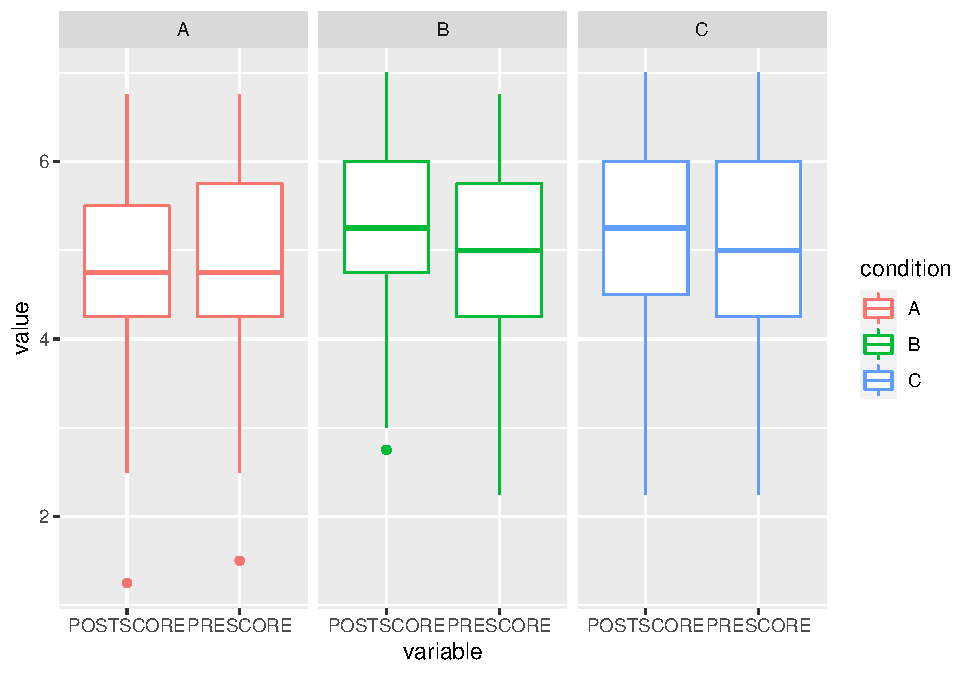
\includegraphics{Thesis-draft-2-w-refs_files/figure-latex/unnamed-chunk-1-1.pdf}

Descriptive statistics are summarized in table 1 above. Our data was
analyzed using a 2x3 ANOVA with one within subjects factor (time of
measurement, pre or post intervention) and one between subjects factor
(experimental intervention type). Our main effect for our `passive'
intervention was not significant (p \textgreater{} .05) with our
estimate being that participants in the passive intervention having
greater support for UHC than those in the control condition. Our main
effect for our `active' intervention was also not significant (p
\textgreater{} .05) with our estimate being that participants in the
active intervention having greater support for UHC than those in the
control condition as well.

There was a significant interaction for the effect of time and our
intervention. Participants only had an increase in support for UHC from
pre to post measure when they were assigned to one of the two
intervention conditions, specifically the interaction between being
assigned to our passive intervention (condition C), and the
post-intervention measure of support for UHC (p = 0.095).

Looking at our graph, we see in our box and whisker plot, that there
does seem to be a trend towards increased scores on support for UHC from
the pre to the post for our two experimental interventions. Just as
importantly, we also see a strong lack of change from pre to post
intervention support for UHC in our control condition.

\hypertarget{bayesian-methods}{%
\subsection{Bayesian Methods}\label{bayesian-methods}}

\begin{Shaded}
\begin{Highlighting}[]
\KeywordTok{summary}\NormalTok{(m8)}
\end{Highlighting}
\end{Shaded}

\begin{verbatim}
##  Family: cumulative 
##   Links: mu = logit; disc = identity 
## Formula: measurement ~ condition * time + (1 | SUBJECT) 
##    Data: UHC_final_long (Number of observations: 1472) 
## Samples: 4 chains, each with iter = 2000; warmup = 1000; thin = 1;
##          total post-warmup samples = 4000
## 
## Group-Level Effects: 
## ~SUBJECT (Number of levels: 184) 
##               Estimate Est.Error l-95% CI u-95% CI Rhat Bulk_ESS Tail_ESS
## sd(Intercept)     1.84      0.12     1.62     2.07 1.00     1130     2257
## 
## Population-Level Effects: 
##                    Estimate Est.Error l-95% CI u-95% CI Rhat Bulk_ESS Tail_ESS
## Intercept[1]          -4.93      0.33    -5.58    -4.29 1.01     1117     1927
## Intercept[2]          -3.41      0.29    -3.97    -2.86 1.01      936     1736
## Intercept[3]          -2.12      0.27    -2.65    -1.58 1.01      860     1576
## Intercept[4]          -0.70      0.27    -1.22    -0.17 1.01      841     1404
## Intercept[5]           0.63      0.27     0.11     1.16 1.01      849     1459
## Intercept[6]           2.60      0.27     2.06     3.14 1.01      909     1641
## conditionB             0.55      0.37    -0.18     1.28 1.01      793     1486
## conditionC             0.65      0.36    -0.08     1.37 1.01      768     1523
## timepre               -0.15      0.16    -0.46     0.17 1.00     3062     3104
## conditionB:timepre    -0.12      0.23    -0.56     0.31 1.00     3561     3608
## conditionC:timepre    -0.22      0.23    -0.68     0.23 1.00     3433     3319
## 
## Samples were drawn using sampling(NUTS). For each parameter, Bulk_ESS
## and Tail_ESS are effective sample size measures, and Rhat is the potential
## scale reduction factor on split chains (at convergence, Rhat = 1).
\end{verbatim}

\begin{Shaded}
\begin{Highlighting}[]
\KeywordTok{marginal_effects}\NormalTok{(m8, }\StringTok{"condition"}\NormalTok{, }\DataTypeTok{ordinal =} \OtherTok{TRUE}\NormalTok{)}
\end{Highlighting}
\end{Shaded}

\begin{verbatim}
## Warning: Method 'marginal_effects' is deprecated. Please use
## 'conditional_effects' instead.
\end{verbatim}

\begin{verbatim}
## Warning: Argument 'ordinal' is deprecated. Please use 'categorical' instead.
\end{verbatim}

\includegraphics{Thesis-draft-2-w-refs_files/figure-latex/unnamed-chunk-2-1.pdf}

Descriptive statistics are summarized in table 2 above. Our data was
analyzed using a 2x3 ANOVA with one within subjects factor (time of
measurement, pre or post intervention) and one between subjects factor
(experimental intervention type). Being in condition B vs A has a 71.6\%
increase in the odds of seeing support for UHC increase by a point.
Being in condition B vs A increases probability of improving support for
UHC by a point by a maximum of 13.5\%. Being in condition C vs A has a
95.4\% increase in the odds of seeing support for UHC increase by a
point. Being in condition C vs A increases probability of improving
support for UHC by a point by a maximum of 16.75\%. Looking at the
variable that represents Pre scores for all conditions, the estimates
for all the values are all negative, and roughly the same. Thus, I would
consider all pre-test values to have lower scores than all post test
values. There seems to be a moderate amount of uncertainty for the odds
ratios of all our conclusions, excepting our interaction between
condition C and postscore, which has a small amount of uncertainty.

Looking at our graph, we see in our ``heatmap'', that there does seem to
be a trend towards increased scores on support for UHC from the pre to
the post for our two experimental interventions. We can see this by
looking at the increased probability of higher scores in the two
intervention categories.

\hypertarget{pilot-conclusion}{%
\section{Pilot Conclusion}\label{pilot-conclusion}}

\hypertarget{summary-of-pilot-study-results}{%
\subsection{Summary of Pilot Study
Results}\label{summary-of-pilot-study-results}}

The initial problem we were examining was how we could improve support
for Universal Health Care. The method we landed on was exposing
participants to an explicit health benefit package through either an
informational intervention, or an experiential intervention. Our first
hypothesis was that exposure to an explicit health benefit package will
improve support for UHC as compared to a control. Our second hypothesis
was that the impact of exposure to an HBP on support for UHC would be
moderated by whether the exposure was informational or experiential.
From our frequentist methods, we found no statistically evidence at an
alpha of 0.05 confirming either of our hypothesis. There was an
interaction that trended towards statistical significance between our
time measure and our intervention condition, which provides some support
for our first hypothesis. Looking at our data using Bayesian modeling,
we find that there is weak evidence supporting our first hypothesis,
with a significant amount of uncertainty with our point estimate.
Lastly, our simple two-sample t-test found no difference between our two
intervention conditions, B and C, when seeing which group would
accept/reject the proposed health benefit plan for themselves.

One concern that arose while running our experiment was that our control
condition did not contribute any external validity. Because of this, we
chose to change our `control' condition in our planned study to more
closely reflect `standard' UHC messaging that subjects would see in the
world around them, instead of a filler `dummy' exercise.

Additionally, in the qualitative response section, we found that
participants occasionally had difficulty understanding the instructions.
Several occasions occurred where the participant asked the administrator
how to complete the exercise, after being exposed to the instructions.
Taken all together, we found that improving our instructions and
potentially clarifying or simplifying the task was important before
implementation of our actual study. For these purposes, we chose to then
adapt the pencil and paper exercise into a web-form for ease of use.

\hypertarget{proposed-method}{%
\section{Proposed Method}\label{proposed-method}}

\hypertarget{participants-1}{%
\subsection{Participants}\label{participants-1}}

Our participants will be students enrolled in the Psychology 1000 course
at a large midwestern university. The study fulfills 1 credit
requirement for students in the course, of which students were required
to obtain 7 credit hours. Participants are not given any other incentive
for participation in the study. Participants are randomized into
different conditions within the online survey software used to
administer the pre and post test measures. We hope to have a total
number of participants around 200. This study will be advertised on the
university credit hours tracking software alongside other qualifying
studies, but will receive no other advertisement.

\hypertarget{materials-1}{%
\subsection{Materials}\label{materials-1}}

Each participant begins by being seated at a computer cubicle with
running the online survey software ``Qualtrics'', which is used to
deliver the pre and post test measures, instructions on how to complete
the measures, as well as the condition exercise. Our only pre-test
measure will be a single measure of support for universal health care
(UHC). This is a 4 item measure of support for UHC, adapted from Shen \&
Labouff (2013) that is taken as a simple average, with the third item
reverse scored. Compared to our pilot study, each item was selected
using a sliding scale that went from 0 (strongly disagree) to 100
(strongly agree).

Next, participants in our intervention condition will be directed to a
web-exercise adapted from the Choosing Healthplans All Together (CHAT)
paradigm developed by Danis, Biddle \& Goold (2002). This exercise
consists of participants `filling out' a game board by spending up to 49
`points' in a maximum of 79 spaces. Several groups of medical care are
represented by costing different amounts of points, with some groups
having up to two greater levels of intensity offered for correspondingly
higher amounts of points. The core of the exercise consists of the
trading off of limited funds in order to determine priorities for the
health care system and considering how the specifics of a given plan
would affect individual health outcomes. As compared to the pilot study,
the web-exercise for our intervention condition requires no mathematical
calculation and is much simpler to administer. Our control condition
replaces the `hands on' task of the web-exercise with exposure to
`traditional' messaging on the benefits of UHC, as presented from
trusted sources such as the World Bank and the World Health
Organization. For either condition, the subjects are asked to consider
how the universal health care would affect their own lives.

Lastly, our participants will receive a post-test measure, that consists
of two main items. The first is a post-test measure of support for UHC,
using the Shen et al.~(2013) measurement tool. The second item is
demographic information, including sex, age, and current year of
schooling.

\hypertarget{design-1}{%
\subsection{Design}\label{design-1}}

The design of this experiment is best described by a multi-level model.
Our multi level structure consisted of UHC measures (either pre or post
intervention), nested within each subject. The experiment was thus a 2x2
between subjects design. While our time variable (pre or post
intervention) is `within' our subjects, any given subject will only be
exposed to one of the experimental conditions, thus it is `between'
subjects. The first `2' is our independent variables of time of
measurement (pre or post intervention), the second `2' is our two
experimental conditions, the control and the intervention. Our dependent
variable was support for UHC. I believe that there should be no
extraneous variables that might influence our results.

\hypertarget{procedure-1}{%
\subsection{Procedure}\label{procedure-1}}

The study begins by our administrator requesting that all subjects turn
off personal electronic devices, in order to minimize distraction and
disruption. Next, the subjects are lead by the administrator into the
room, and are briefly told that the study will consist of a computer
survey, with a computer activity during the middle of the survey. Each
subject is then brought to a single-occupant cubicle with a computer
running our Qualtrics survey. At this point, participants are told to
read the instructions carefully, and notify the administrator once the
survey assigned them to an experimental condition. Our subjects at this
point complete the first half of the survey, consisting of our pre-test
measure. After this is completed, the Qualtrics software randomly
assigns the survey participant to one of two experimental conditions,
with instructions on how to complete the computer exercise displayed
upon the screen. Once this occurs, the administrator brings reference
materials to our intervention condition, and both groups of subjects
will complete the exercise after a brief verbal reminder of the task
they were to be working on. After the task is complete, the subject
responds to our post-test measures. Lastly, the subject reads a one page
paper debriefing them of the purpose and theory behind the research, and
is then granted 1 credit in the Psych 1000 system. This entire process
should take 20-25 minutes on average, as evinced in our pilot study.

\hypertarget{modelling}{%
\subsection{Modelling}\label{modelling}}

I plan to employ two sets of models. One standard frequentist model,
accounting for the multi-level nested nature of our repeated measures.
Our other model will be a Bayesian model. A special model detail of
importance is choosing a prior for our cumulative multinomial
regression, of a normal distribution with a mean of zero, and a variance
of 4. This was chosen so as to mimic the nature of our log-odds being
akin to a z-score, with ranges outside of 4 not having much meaning than
one at 2.5. Our main results that we will attend to will be seeing if
the variables that we have hypothesized having an effect on support for
UHC are statistically sigificant, and from the Bayesian perspective,
seeing how much uncertainty we see in our estimates.

\hypertarget{discussion}{%
\section{Discussion}\label{discussion}}

\hypertarget{relate-results-to-past-research}{%
\subsection{Relate Results to Past
Research}\label{relate-results-to-past-research}}

Looking at our pilot study. our expectation was that there would be a
strong effect confirming our hypothesis as our work related strongly to
previous research in the field. We did find a slight effect when
exposing individuals to HBP, but there was significant uncertainty
regarding our result. Keeping in track with previous research, we did
find that overall there was a reasonable level of support for UHC as the
majority of our participants found the plan acceptable. We also
replicated the generally positive level of support found by Huebner et
al. (2006), but in a non-medical student population. With regards to
likelihood of wanting the referenced plans for themselves, the slight
positive result we obtained cleanly replicates the findings of Danis,
Biddle \& Goold, 2002. The majority individuals exposed to a health
benefit package would be willing to use the health package for
themselves. Lastly, our results were different from Weiger, Armstrong \&
Shaffer, 2019. According to Weiger et al.~we should have expected a
stronger effect with the experiential intervention as compared to the
informational intervention. We neither saw a difference in support
between our two interventions (as compared to each other, not the
control), as well as no difference in likelihood to accept the proposed
HBP for self use. However, we may find different results with an
informational intervention that reflects commonly shared information
about UHC, as with our currently proposed study, as compared to the
informational intervention we used in our pilot. Lastly, since there was
a lack of conclusiveness, there is the possibility that the mechanism
underlying opposition to UHC could be different than the initial two we
hypothesized. While an HBP solves very neatly the issue of `fairness'
and `lack of explicit definition' for the program, if opposition to UHC
is due to another issue, it may not ameliorate the problem. Due to this
lack of conclusiveness, there is significant value in the partial
replication we are proposing.

\hypertarget{limitations}{%
\section{Limitations}\label{limitations}}

Both our pilot study and planned study recruited or will recruit
participants from a large midwestern university located in a medium
sized midwestern city. This is not necessarily reflective of the
majority of the insurance buying population, or those individuals able
to effect change on UHC. In addition, our methodology, specifically the
process of instructing our participants how to complete the pencil and
paper exercise in the pilot study, was imperfect. In the free response
portion of the exit survey as well as when administering the experiment,
participants often had trouble understanding the instructions.
Furthermore, our control condition in our pilot was a `dummy exercise',
and we never presented supporting information for UHC using the
`standard' format or content that health organizations would use,
reducing our external validity.

\hypertarget{appendix}{%
\section{Appendix}\label{appendix}}

\hypertarget{pilot-study-code-for-frequentist-mlm---treating-ordinal-values-as-continuous}{%
\subsection{Pilot Study Code for Frequentist MLM - treating ordinal
values as
continuous}\label{pilot-study-code-for-frequentist-mlm---treating-ordinal-values-as-continuous}}

The goal of this analysis is to examine my Universal Health Care benefit
package data with an eye towards considering it as a multilevel model.
The multilevel structure in this study is that each subject has two
support for UHC measurements, one done as a pre-test measure, and one
done as a post-test measure. Thus, our two trial times are nested within
subjects. Our main level two predictor variable is which condition out
of three our subjects were assigned to. We chose the first model
assuming that we would best predict UHC support through a specific
subject, and which condition they were assigned. This model failed to
converge. We next moved to a model that predicted UHC support from just
condition, and it was able to converge. We then wished to examine our
interaction between time, and condition, as that was part of our
hypothesis originally. The model for this also converged. We lastly
tried a more complex model that allowed the intercept to vary by time,
but the model did not converge, thus we returned to analyzing the
results of model 3.

First model, predicting UHC support by subject, and condition, letting
intercepts vary by subject.

m1\textless-lmer(value \textasciitilde{} SUBJECT + condition +
(1\textbar SUBJECT), data = UHC\_final)

We move to this model, as the previous one registered errors.

m2\textless-lmer(value \textasciitilde{} condition +
(1\textbar SUBJECT), data = UHC\_final)

We lastly use this model, as we wish to consider the effect of time as
well as condition.

m3\textless-lmer(value \textasciitilde{} condition*variable +
(1\textbar SUBJECT), data = UHC\_final)

We try both this more complex model, but we failure to converge, so we
return to using m3.

m5\textless-lmer(value \textasciitilde{} condition*variable +
(1\textbar SUBJECT) + (1\textbar variable), data = UHC\_final)

\hypertarget{pilot-study-code-for-bayesian-mlm---treating-ordinal-values-as-ordinal}{%
\section{Pilot Study Code for Bayesian MLM - Treating ordinal values as
ordinal}\label{pilot-study-code-for-bayesian-mlm---treating-ordinal-values-as-ordinal}}

To analyze the data in a different way, I have chosen to look at the
per-item scores in the aggregated measure of support for UHC. Treating
these values as ordinal, I reshaped my data from wide to tall, with each
pre and post test question recieving it's own row. I chose to set my
prior based on the understanding that the variance range should roughly
mimic z-scores, with values of +- 2.5 being near the edge of the range.

I started with a simple model, and added more complexity as I desired to
test my hypothesis. The first model was a simple affect of condition,
time, and question. After finding that the question parameter did not
make much of an impact, I chose to look at the interaction between
condition and time, something I presupposed would have an effect. The
last model I examined had a random intercept by subject, but also
allowed the slope for `condition' to vary by subject. Sadly, this model
refused to converge and thus I decided to use my m8 model.

Create a prior based on our understanding of likely ranges in a Z-score.

myprior\textless-prior(normal(0,2.5), class =``Intercept'')

Simplest form of our model.

m7\textless-brm(measurement \textasciitilde{} condition + time +
question + (1\textbar SUBJECT), data = UHC\_final\_long, family =
cumulative(``logit''), prior = myprior)

Simplest form testing our base hypothesis.

m8\textless-brm(measurement \textasciitilde{} condition*time +
(1\textbar SUBJECT), data = UHC\_final\_long, family =
cumulative(``logit''), prior = myprior)

Model that did not converge

m9\textless-brm(measurement \textasciitilde{} condition*time +
(condition\textbar SUBJECT), data = UHC\_final\_long, family =
cumulative(``logit''), prior = myprior)

\hypertarget{references}{%
\section*{References}\label{references}}
\addcontentsline{toc}{section}{References}

\hypertarget{refs}{}
\leavevmode\hypertarget{ref-Assembly1991}{}%
Assembly, The General. 1991. ``UN general assembly resolution 44/225.''
\emph{Marine Policy} 15 (5): 331--32.
\url{https://doi.org/10.1016/0308-597x(91)90085-p}.

\leavevmode\hypertarget{ref-Chalkidou2014}{}%
Chalkidou, Kalipso, Patricio Marquez, Preet K. Dhillon, Yot
Teerawattananon, Thunyarat Anothaisintawee, Carlos Augusto Grabois
Gadelha, and Richard Sullivan. 2014. ``Evidence-informed frameworks for
cost-effective cancer care and prevention in low, middle, and
high-income countries.'' \emph{The Lancet Oncology} 15 (3): e119--e131.
\url{https://doi.org/10.1016/S1470-2045(13)70547-3}.

\leavevmode\hypertarget{ref-Danis2002}{}%
Danis, Marion, Andrea K. Biddle, and Susan Dorr Goold. 2002. ``Insurance
benefit preferences of the low-income uninsured.'' \emph{Journal of
General Internal Medicine} 17 (2): 125--33.
\url{https://doi.org/10.1046/j.1525-1497.2002.10609.x}.

\leavevmode\hypertarget{ref-Danis2004}{}%
Danis, Marion, Andrea K. Biddle, and Susan Dorr Goold. 2004. ``Enrollees
Choose Priorities for Medicare.'' \emph{Gerontologist} 44 (1): 58--67.
\url{https://doi.org/10.1093/geront/44.1.58}.

\leavevmode\hypertarget{ref-Galvani2017}{}%
Galvani, Alison P, David P Durham, Sten H Vermund, and Meagan C
Fitzpatrick. 2017. ``California Universal Health Care: An economic
stimulus and lifesaving proposal.'' \emph{The Lancet} 390 (10106):
2012--4. \url{https://doi.org/10.1016/S0140-6736(17)32148-7.California}.

\leavevmode\hypertarget{ref-Glassman2016}{}%
Glassman, Amanda, Ursula Giedion, Yuna Sakuma, and Peter C. Smith. 2016.
``Defining a health benefits package: What are the necessary
processes?'' \emph{Health Systems and Reform} 2 (1): 39--50.
\url{https://doi.org/10.1080/23288604.2016.1124171}.

\leavevmode\hypertarget{ref-Goold2005}{}%
Goold, Susan Dorr, Andrea K. Biddle, Glenn Klipp, Charles N. Hall, and
Marion Danis. 2005. ``Choosing healthplans all together: A deliberative
exercise for allocating limited health care resources.'' \emph{Journal
of Health Politics, Policy and Law} 30 (4): 563--601.
\url{https://doi.org/10.1215/03616878-30-4-563}.

\leavevmode\hypertarget{ref-Huebner2006}{}%
Huebner, Jeffrey, Jaya R. Agrawal, Ashwini R. Sehgal, Paul Jung, Joan
Hedgecock, and Steven R. Simon. 2006. ``Universal health care and reform
of the health care system: Views of medical students in the United
States.'' \emph{Academic Medicine} 81 (8): 721--27.
\url{https://doi.org/10.1097/00001888-200608000-00008}.

\leavevmode\hypertarget{ref-Hurst2018}{}%
Hurst, Samia A., Mélinée Schindler, Susan D. Goold, and Marion Danis.
2018. ``Swiss-CHAT: Citizens discuss priorities for Swiss health
insurance coverage.'' \emph{International Journal of Health Policy and
Management} 7 (8): 746--54.
\url{https://doi.org/10.15171/ijhpm.2018.15}.

\leavevmode\hypertarget{ref-Manchikanti2010}{}%
Manchikanti, Laxmaiah, Frank J. E. Falco, Mark V. Boswell, and Joshua A.
Hirsch. 2010. ``Facts, fallacies, and politics of comparative
effectiveness research: Part 2 - Implications for interventional pain
management.'' \emph{Pain Physician} 13 (1): 55--80.

\leavevmode\hypertarget{ref-Manchikanti2009}{}%
Manchikanti, Laxmaiah, Vijay Singh, Sukdeb Datta, Steven P. Cohen, and
Joshua A. Hirsch. 2009. ``Comprehensive review of epidemiology, scope,
and impact of spinal pain.'' \emph{Pain Physician} 12 (4): 35--70.

\leavevmode\hypertarget{ref-Panpiemras2011}{}%
Panpiemras, Jirawat, Thitima Puttitanun, Krislert Samphantharak, and
Kannika Thampanishvong. 2011. ``Impact of Universal Health Care Coverage
on patient demand for health care services in Thailand.'' \emph{Health
Policy} 103 (2-3): 228--35.
\url{https://doi.org/10.1016/j.healthpol.2011.08.008}.

\leavevmode\hypertarget{ref-Shen2016}{}%
Shen, Megan Johnson, and Jordan P. Labouff. 2016. ``More than political
ideology: Subtle racial prejudice as a predictor of opposition to
universal health care among U.S. Citizens.'' \emph{Journal of Social and
Political Psychology} 4 (2): 493--520.
\url{https://doi.org/10.5964/jspp.v4i2.245}.

\leavevmode\hypertarget{ref-Summers2015}{}%
Summers, Lawrence H. 2015. ``Economists' declaration on universal health
coverage.'' \emph{The Lancet} 386 (10008): 2112--3.
\url{https://doi.org/10.1016/S0140-6736(15)00242-1}.

\leavevmode\hypertarget{ref-Wegier2019}{}%
Wegier, Pete, and Victoria A. Shaffer. 2018. ``Corrigendum to `Aiding
risk information learning through simulated experience (ARISE): Using
simulated outcomes to improve understanding of conditional probabilities
in prenatal Down syndrome screening' {[}Patient Educ. Counselling 100
(October (10)) (2017).''
\url{https://doi.org/10.1016/j.pec.2017.12.001}.

\end{document}
